
%% bare_conf.tex
%% V1.3
%% 2007/01/11
%% by Michael Shell
%% See:
%% http://www.michaelshell.org/
%% for current contact information.
%%
%% This is a skeleton file demonstrating the use of IEEEtran.cls
%% (requires IEEEtran.cls version 1.7 or later) with an IEEE conference paper.
%%
%% Support sites:
%% http://www.michaelshell.org/tex/ieeetran/
%% http://www.ctan.org/tex-archive/macros/latex/contrib/IEEEtran/
%% and
%% http://www.ieee.org/

%%*************************************************************************
%% Legal Notice:
%% This code is offered as-is without any warranty either expressed or
%% implied; without even the implied warranty of MERCHANTABILITY or
%% FITNESS FOR A PARTICULAR PURPOSE! 
%% User assumes all risk.
%% In no event shall IEEE or any contributor to this code be liable for
%% any damages or losses, including, but not limited to, incidental,
%% consequential, or any other damages, resulting from the use or misuse
%% of any information contained here.
%%
%% All comments are the opinions of their respective authors and are not
%% necessarily endorsed by the IEEE.
%%
%% This work is distributed under the LaTeX Project Public License (LPPL)
%% ( http://www.latex-project.org/ ) version 1.3, and may be freely used,
%% distributed and modified. A copy of the LPPL, version 1.3, is included
%% in the base LaTeX documentation of all distributions of LaTeX released
%% 2003/12/01 or later.
%% Retain all contribution notices and credits.
%% ** Modified files should be clearly indicated as such, including  **
%% ** renaming them and changing author support contact information. **
%%
%% File list of work: IEEEtran.cls, IEEEtran_HOWTO.pdf, bare_adv.tex,
%%                    bare_conf.tex, bare_jrnl.tex, bare_jrnl_compsoc.tex
%%*************************************************************************

% *** Authors should verify (and, if needed, correct) their LaTeX system  ***
% *** with the testflow diagnostic prior to trusting their LaTeX platform ***
% *** with production work. IEEE's font choices can trigger bugs that do  ***
% *** not appear when using other class files.                            ***
% The testflow support page is at:
% http://www.michaelshell.org/tex/testflow/



% Note that the a4paper option is mainly intended so that authors in
% countries using A4 can easily print to A4 and see how their papers will
% look in print - the typesetting of the document will not typically be
% affected with changes in paper size (but the bottom and side margins will).
% Use the testflow package mentioned above to verify correct handling of
% both paper sizes by the user's LaTeX system.
%
% Also note that the "draftcls" or "draftclsnofoot", not "draft", option
% should be used if it is desired that the figures are to be displayed in
% draft mode.
%
\documentclass[10pt, conference, compsocconf]{IEEEtran}
% Add the compsocconf option for Computer Society conferences.
%
% If IEEEtran.cls has not been installed into the LaTeX system files,
% manually specify the path to it like:
% \documentclass[conference]{../sty/IEEEtran}





% Some very useful LaTeX packages include:
% (uncomment the ones you want to load)


% *** MISC UTILITY PACKAGES ***
%
%\usepackage{ifpdf}
% Heiko Oberdiek's ifpdf.sty is very useful if you need conditional
% compilation based on whether the output is pdf or dvi.
% usage:
% \ifpdf
%   % pdf code
% \else
%   % dvi code
% \fi
% The latest version of ifpdf.sty can be obtained from:
% http://www.ctan.org/tex-archive/macros/latex/contrib/oberdiek/
% Also, note that IEEEtran.cls V1.7 and later provides a builtin
% \ifCLASSINFOpdf conditional that works the same way.
% When switching from latex to pdflatex and vice-versa, the compiler may
% have to be run twice to clear warning/error messages.






% *** CITATION PACKAGES ***
%
%\usepackage{cite}
% cite.sty was written by Donald Arseneau
% V1.6 and later of IEEEtran pre-defines the format of the cite.sty package
% \cite{} output to follow that of IEEE. Loading the cite package will
% result in citation numbers being automatically sorted and properly
% "compressed/ranged". e.g., [1], [9], [2], [7], [5], [6] without using
% cite.sty will become [1], [2], [5]--[7], [9] using cite.sty. cite.sty's
% \cite will automatically add leading space, if needed. Use cite.sty's
% noadjust option (cite.sty V3.8 and later) if you want to turn this off.
% cite.sty is already installed on most LaTeX systems. Be sure and use
% version 4.0 (2003-05-27) and later if using hyperref.sty. cite.sty does
% not currently provide for hyperlinked citations.
% The latest version can be obtained at:
% http://www.ctan.org/tex-archive/macros/latex/contrib/cite/
% The documentation is contained in the cite.sty file itself.






% *** GRAPHICS RELATED PACKAGES ***
%
\ifCLASSINFOpdf
  \usepackage[pdftex]{graphicx}
  % declare the path(s) where your graphic files are
  \graphicspath{{./res/}}
  % and their extensions so you won't have to specify these with
  % every instance of \includegraphics
  \DeclareGraphicsExtensions{.pdf,.jpeg,.png}
\else
  % or other class option (dvipsone, dvipdf, if not using dvips). graphicx
  % will default to the driver specified in the system graphics.cfg if no
  % driver is specified.
  % \usepackage[dvips]{graphicx}
  % declare the path(s) where your graphic files are
  % \graphicspath{{../eps/}}
  % and their extensions so you won't have to specify these with
  % every instance of \includegraphics
  % \DeclareGraphicsExtensions{.eps}
\fi
% graphicx was written by David Carlisle and Sebastian Rahtz. It is
% required if you want graphics, photos, etc. graphicx.sty is already
% installed on most LaTeX systems. The latest version and documentation can
% be obtained at: 
% http://www.ctan.org/tex-archive/macros/latex/required/graphics/
% Another good source of documentation is "Using Imported Graphics in
% LaTeX2e" by Keith Reckdahl which can be found as epslatex.ps or
% epslatex.pdf at: http://www.ctan.org/tex-archive/info/
%
% latex, and pdflatex in dvi mode, support graphics in encapsulated
% postscript (.eps) format. pdflatex in pdf mode supports graphics
% in .pdf, .jpeg, .png and .mps (metapost) formats. Users should ensure
% that all non-photo figures use a vector format (.eps, .pdf, .mps) and
% not a bitmapped formats (.jpeg, .png). IEEE frowns on bitmapped formats
% which can result in "jaggedy"/blurry rendering of lines and letters as
% well as large increases in file sizes.
%
% You can find documentation about the pdfTeX application at:
% http://www.tug.org/applications/pdftex





% *** MATH PACKAGES ***
%
%\usepackage[cmex10]{amsmath}
% A popular package from the American Mathematical Society that provides
% many useful and powerful commands for dealing with mathematics. If using
% it, be sure to load this package with the cmex10 option to ensure that
% only type 1 fonts will utilized at all point sizes. Without this option,
% it is possible that some math symbols, particularly those within
% footnotes, will be rendered in bitmap form which will result in a
% document that can not be IEEE Xplore compliant!
%
% Also, note that the amsmath package sets \interdisplaylinepenalty to 10000
% thus preventing page breaks from occurring within multiline equations. Use:
%\interdisplaylinepenalty=2500
% after loading amsmath to restore such page breaks as IEEEtran.cls normally
% does. amsmath.sty is already installed on most LaTeX systems. The latest
% version and documentation can be obtained at:
% http://www.ctan.org/tex-archive/macros/latex/required/amslatex/math/





% *** SPECIALIZED LIST PACKAGES ***
%
%\usepackage{algorithmic}
% algorithmic.sty was written by Peter Williams and Rogerio Brito.
% This package provides an algorithmic environment fo describing algorithms.
% You can use the algorithmic environment in-text or within a figure
% environment to provide for a floating algorithm. Do NOT use the algorithm
% floating environment provided by algorithm.sty (by the same authors) or
% algorithm2e.sty (by Christophe Fiorio) as IEEE does not use dedicated
% algorithm float types and packages that provide these will not provide
% correct IEEE style captions. The latest version and documentation of
% algorithmic.sty can be obtained at:
% http://www.ctan.org/tex-archive/macros/latex/contrib/algorithms/
% There is also a support site at:
% http://algorithms.berlios.de/index.html
% Also of interest may be the (relatively newer and more customizable)
% algorithmicx.sty package by Szasz Janos:
% http://www.ctan.org/tex-archive/macros/latex/contrib/algorithmicx/




% *** ALIGNMENT PACKAGES ***
%
%\usepackage{array}
% Frank Mittelbach's and David Carlisle's array.sty patches and improves
% the standard LaTeX2e array and tabular environments to provide better
% appearance and additional user controls. As the default LaTeX2e table
% generation code is lacking to the point of almost being broken with
% respect to the quality of the end results, all users are strongly
% advised to use an enhanced (at the very least that provided by array.sty)
% set of table tools. array.sty is already installed on most systems. The
% latest version and documentation can be obtained at:
% http://www.ctan.org/tex-archive/macros/latex/required/tools/


%\usepackage{mdwmath}
%\usepackage{mdwtab}
% Also highly recommended is Mark Wooding's extremely powerful MDW tools,
% especially mdwmath.sty and mdwtab.sty which are used to format equations
% and tables, respectively. The MDWtools set is already installed on most
% LaTeX systems. The lastest version and documentation is available at:
% http://www.ctan.org/tex-archive/macros/latex/contrib/mdwtools/


% IEEEtran contains the IEEEeqnarray family of commands that can be used to
% generate multiline equations as well as matrices, tables, etc., of high
% quality.


%\usepackage{eqparbox}
% Also of notable interest is Scott Pakin's eqparbox package for creating
% (automatically sized) equal width boxes - aka "natural width parboxes".
% Available at:
% http://www.ctan.org/tex-archive/macros/latex/contrib/eqparbox/





% *** SUBFIGURE PACKAGES ***
%\usepackage[tight,footnotesize]{subfigure}
% subfigure.sty was written by Steven Douglas Cochran. This package makes it
% easy to put subfigures in your figures. e.g., "Figure 1a and 1b". For IEEE
% work, it is a good idea to load it with the tight package option to reduce
% the amount of white space around the subfigures. subfigure.sty is already
% installed on most LaTeX systems. The latest version and documentation can
% be obtained at:
% http://www.ctan.org/tex-archive/obsolete/macros/latex/contrib/subfigure/
% subfigure.sty has been superceeded by subfig.sty.



%\usepackage[caption=false]{caption}
%\usepackage[font=footnotesize]{subfig}
% subfig.sty, also written by Steven Douglas Cochran, is the modern
% replacement for subfigure.sty. However, subfig.sty requires and
% automatically loads Axel Sommerfeldt's caption.sty which will override
% IEEEtran.cls handling of captions and this will result in nonIEEE style
% figure/table captions. To prevent this problem, be sure and preload
% caption.sty with its "caption=false" package option. This is will preserve
% IEEEtran.cls handing of captions. Version 1.3 (2005/06/28) and later 
% (recommended due to many improvements over 1.2) of subfig.sty supports
% the caption=false option directly:
%\usepackage[caption=false,font=footnotesize]{subfig}
%
% The latest version and documentation can be obtained at:
% http://www.ctan.org/tex-archive/macros/latex/contrib/subfig/
% The latest version and documentation of caption.sty can be obtained at:
% http://www.ctan.org/tex-archive/macros/latex/contrib/caption/




% *** FLOAT PACKAGES ***
%
%\usepackage{fixltx2e}
% fixltx2e, the successor to the earlier fix2col.sty, was written by
% Frank Mittelbach and David Carlisle. This package corrects a few problems
% in the LaTeX2e kernel, the most notable of which is that in current
% LaTeX2e releases, the ordering of single and double column floats is not
% guaranteed to be preserved. Thus, an unpatched LaTeX2e can allow a
% single column figure to be placed prior to an earlier double column
% figure. The latest version and documentation can be found at:
% http://www.ctan.org/tex-archive/macros/latex/base/



%\usepackage{stfloats}
% stfloats.sty was written by Sigitas Tolusis. This package gives LaTeX2e
% the ability to do double column floats at the bottom of the page as well
% as the top. (e.g., "\begin{figure*}[!b]" is not normally possible in
% LaTeX2e). It also provides a command:
%\fnbelowfloat
% to enable the placement of footnotes below bottom floats (the standard
% LaTeX2e kernel puts them above bottom floats). This is an invasive package
% which rewrites many portions of the LaTeX2e float routines. It may not work
% with other packages that modify the LaTeX2e float routines. The latest
% version and documentation can be obtained at:
% http://www.ctan.org/tex-archive/macros/latex/contrib/sttools/
% Documentation is contained in the stfloats.sty comments as well as in the
% presfull.pdf file. Do not use the stfloats baselinefloat ability as IEEE
% does not allow \baselineskip to stretch. Authors submitting work to the
% IEEE should note that IEEE rarely uses double column equations and
% that authors should try to avoid such use. Do not be tempted to use the
% cuted.sty or midfloat.sty packages (also by Sigitas Tolusis) as IEEE does
% not format its papers in such ways.





% *** PDF, URL AND HYPERLINK PACKAGES ***
%
%\usepackage{url}
% url.sty was written by Donald Arseneau. It provides better support for
% handling and breaking URLs. url.sty is already installed on most LaTeX
% systems. The latest version can be obtained at:
% http://www.ctan.org/tex-archive/macros/latex/contrib/misc/
% Read the url.sty source comments for usage information. Basically,
% \url{my_url_here}.





% *** Do not adjust lengths that control margins, column widths, etc. ***
% *** Do not use packages that alter fonts (such as pslatex).         ***
% There should be no need to do such things with IEEEtran.cls V1.6 and later.
% (Unless specifically asked to do so by the journal or conference you plan
% to submit to, of course. )


% correct bad hyphenation here
\hyphenation{op-tical net-works semi-conduc-tor}


\begin{document}
%
% paper title
% can use linebreaks \\ within to get better formatting as desired
\title{Methods of Detecting Home Language Shift in Canadian Census Data}


% author names and affiliations
% use a multiple column layout for up to two different
% affiliations

\author{\IEEEauthorblockN{Chris Choy, Kiefer Co, Matthew Fogel, Clarke Garrioch and Katie Martchenko}
\IEEEauthorblockA{Department of Computer Science\\
University of Manitoba\\
Winnipeg, MB, Canada\\
Email: kleung@cs.umanitoba.ca}
}

% conference papers do not typically use \thanks and this command
% is locked out in conference mode. If really needed, such as for
% the acknowledgment of grants, issue a \IEEEoverridecommandlockouts
% after \documentclass

% for over three affiliations, or if they all won't fit within the width
% of the page, use this alternative format:
% 
%\author{\IEEEauthorblockN{Michael Shell\IEEEauthorrefmark{1},
%Homer Simpson\IEEEauthorrefmark{2},
%James Kirk\IEEEauthorrefmark{3}, 
%Montgomery Scott\IEEEauthorrefmark{3} and
%Eldon Tyrell\IEEEauthorrefmark{4}}
%\IEEEauthorblockA{\IEEEauthorrefmark{1}School of Electrical and Computer Engineering\\
%Georgia Institute of Technology,
%Atlanta, Georgia 30332--0250\\ Email: see http://www.michaelshell.org/contact.html}
%\IEEEauthorblockA{\IEEEauthorrefmark{2}Twentieth Century Fox, Springfield, USA\\
%Email: homer@thesimpsons.com}
%\IEEEauthorblockA{\IEEEauthorrefmark{3}Starfleet Academy, San Francisco, California 96678-2391\\
%Telephone: (800) 555--1212, Fax: (888) 555--1212}
%\IEEEauthorblockA{\IEEEauthorrefmark{4}Tyrell Inc., 123 Replicant Street, Los Angeles, California 90210--4321}}




% use for special paper notices
%\IEEEspecialpapernotice{(Invited Paper)}




% make the title area
\maketitle


\begin{abstract}
Canada is a nation composed of a highly diverse language population. This provides a unique opportunity to study the factors causing certain languages and language families to be lost over subsequent generations amongst allophones (people with a mother tongue other than English or French). This paper applies and compares the performance of Decision Tree Induction, Random Forest, and Categorical Naive Bayesian algorithm to census microdata to analyze the influence of various social and economic factors on the probability that allophones adopt official languages as their language spoken at home.

\end{abstract}

\begin{IEEEkeywords}
component; language cohorts; allophones; mother tongue; language persistence

\end{IEEEkeywords}


% For peer review papers, you can put extra information on the cover
% page as needed:
% \ifCLASSOPTIONpeerreview
% \begin{center} \bfseries EDICS Category: 3-BBND \end{center}
% \fi
%
% For peerreview papers, this IEEEtran command inserts a page break and
% creates the second title. It will be ignored for other modes.
\IEEEpeerreviewmaketitle



\section{Introduction}
% no \IEEEPARstart
Canada is a nation composed of a highly diverse language population. Immigration and migration has risen both in numbers and as culturally relevant components of modern communities, especially in diverse countries such as Canada.

This provides a unique opportunity to study the rates at which certain languages and language families are lost over subsequent generations as allophones (people with a mother tongue other than English or French) adopt English or French as their primary language. Certain factors such as sex, age, educational status and economic success may prove to be a key indicator of how quickly an individual adopts a language other than their mother tongue in everyday life.

A language shift occurs when an allophone adopts an official language as their primary language, i.e. language spoken at home. Several studies have aimed to measure language shift rates through linear regression on various cohorts of the population. Ultimately, it is impossible to ascertain precisely when a language shift occurs, so the insights offered by linear regression are limited in accuracy.

This paper proposes an application of various data mining algorithms and compares their accuracy and speed when used on census data, namely the Random Forest algorithm, the Decision Tree algorithm, and the Categorical Naive Bayesian algorithm.

Some challenges working with census microdata include the fact that the Public Use Microdata Files (PUMF) have been downsampled from the census population size. In order to perform an analysis that would take into account the population distribution, records are needed to be multiplied by a corresponding weight included in the PUMF datasets. Additionally, the PUMF datasets contain over 100 potential features, some of which contain largely invalid/unavailable data. As a result, some level of feature selection is required.

The Canadian census is conducted every five years. As a result, changes that occur between census periods may not be captured at the exact time of their occurrence.

% You must have at least 2 lines in the paragraph with the drop letter
% (should never be an issue)

\section{Related Work}
Over the past several years, researchers have come up with multiple approaches to analyze census microdata to determine the rates at which allophones express a language shift. Several authors has focused on identifying whether a  shift towards official languages (English and French) have occurred by determining if the mother tongue is the same as the language spoken at home. This is typically accomplished by performing linear regression.

\subsection{Linear Regression of Language Cohorts}
\subsubsection{Fictitious Cohorts}
Patrick Sabourin and Alain Bélanger use the concept of a 'fictitious cohort', in which groups separated by age or time since immigration are compared across a single census. They define language persistence as the proportion of each cohort that has kept their mother tongue as the language most often spoken at home. The authors analyze language shift using linear regression and polynomial regression. They then construct a survival curve which determines the probability that each subsection of a cohort (such as a specific age group) will undergo a language shift. They make the assumption that the rate of language shift is constant among several censuses.
\cite{dynamics1}

One limitation to this method is that members of a cohort are defined in binary terms as having lost a language if they no longer speak it at home, while this process might occur gradually in real time. Additionally, certain language groups may experience different rates of language shift. \cite{dynamics1}

\subsubsection{Synthetic Cohorts}
Marie T Mora, Daniel J Villa and Alberto Davila use an alternative method known as 'synthetic cohort' analysis on census data in the United States. Their paper aims to better understand the recent dynamic of language loss and intergenerational maintenance of Spanish in the U.S., and compare it to other non-English languages. In other words, exploring the retention or loss of Spanish and other non-English speakers in the U.S., particularly among foreign-born and U.S.-born children with immigrant parents. \cite{spanish1}

The technique for analysis, synthetic cohort analysis, is based on data drawn from 1980, 1990, and 2000 United States Censuses. It creates a temporal representation of a population, over ten-year intervals. The authors track the reported language use of individuals starting at ages 5-7 and ending at ages 15-17 across two United States census. This selection is due to children being able to speak at ages 5-7 and languages tending not to be lost after ages 15-17. \cite{spanish1}

This is in contrast to cross-sectional methods which use data from only one Census period to analyze language shifts. Combining this method with the synthetic cohort, the paper argues that the dynamic in language shift is better predicted, supported by what has been observed in the U.S. \cite{spanish1}

There are still some difficulties with this approach. For example, 1980 and 1990 samples could have emigrations before 1990 and 2000, and from this the “true” cohorts of the foreign-born may not be entirely reflected.\cite{spanish1}

\subsubsection{Limitations of Linear Regression}
As seen above, multiple approaches to analyzing language cohorts temporally run into limitations in how census data is collected. Sampling errors and poorly worded census questions make it difficult to capture whether emigration has occurred between censuses. Even within a census, it is tempting to view language shift within a cohort as binary when this process occurs gradually.

Populations are dynamic, and multiple categorical variables influence whether a language that is the mother tongue is spoken at home. A decision tree can reveal which categorical variables determine whether mother tongue is retained as the language spoken at home.

\subsection{Decision Tree Performance in Other Areas}
\subsubsection{Decision Trees in Student Performance Prediction}
Decision trees have also been compared and applied in other fields. Osmanbegovic and Suljic compared the performance of an implementation of a decision tree algorithm, Naive Bayes algorithm, and a Multilayer Perceptron algorithm in predicting student performance by the prediction accuracy, learning time, and error rate. \cite{performance1}

Osmanbegovic and Suljic used 12 input features such as gender, GPA, and whether or not the student had scholarships, and outputted whether or not the student would pass or fail. The output could also be classified by letter grades, but due to the disparity in the amount of data for each class, was not used. \cite{performance1}

They found that the Naive Bayes algorithm managed to outperform the C4.5 decision tree algorithm implementation, J48, in both prediction accuracy, and error rate. Additionally, it was found that the Naive Bayes algorithm and the decision tree algorithm created prediction models that were both accurate, and user-friendly enough for the stakeholders. \cite{performance1}

\subsubsection{Improvements}
Similarly to Osmanbegovic and Suljic's data, some classes in census data are going to have differing amounts of data, and will affect prediction accuracy. Instead of changing the class groupings to get more equal representation, weights could be added to the training data to account for these differences. In the case of the Canadian Census data, these weights are already added to the data for use.

\subsection{An Alternative Approach to Census Data Mining}
In their paper, Klösgen and May took a different approach to mining census data. Klösgen and May used the United Kingdom's census data, which was only available in an aggregated form. The census data was available aggregated across various wards within the region, along with a detailed set of geographic layers. Thus, Klösgen and May decided to use those wards as the focus of their examination, and propose an application of SubgroupMiner, an advanced subgroup mining system. \cite{census1}

\subsection{An Improved Decision Tree Algorithm}
Hulten, Spencer, and Domingos' CVFDT algorithm improves on the VFDT decision tree learner by accounting for data changing over time. \cite{dtrees1} Their CVFDT algorithm works by maintaining a decision tree with respect to a sliding window of data and grows an alternative subtree to replace an old one if it becomes out of date. This allows for it to learn a similar model to one from the VFDT algorithm but in constant time \cite{dtrees1}.

Applying the algorithm to census data seems like a natural fit, and can be used to improve the performance of any decision tree learners in use. The addition of the time aspect could also be used to improve the accuracy in cases where the data from only one period of time is used, instead of multiple.


\section{Methodology}

\subsection{General Process}
% @TODO expand on this
The general process is as follows:
\begin{enumerate}
	\item Determine when a shift in language occurs
	\item Preprocess the data, converting any continuous values into discrete values
	\item Split the data into training and testing sets
	\item Construct the various classifiers, and evaluate them
\end{enumerate}

Due to the nature of decision trees, all continuous values must be converted into a discrete value. Additionally, differences in datasets may result in the definition of language shift needing to be adjusted.

\subsection{Mining the 2016 Canadian Census}
In addition to the general steps stated above, applying them to the 2016 Canadian Census required further work, namely the additional preprocessing due to the format of the data.

The analysis was performed in Python 3 via Jupyter Notebooks.  
The \textbf{Pandas} package was used to import the 2016 PUMF Individuals CSV file as a  \textit{DataFrame} and perform manipulations on the \textit{DataFrame}, described in more detail in the data preprocessing section.

Several modules in the \textbf{scikit-learn} package were used for the classification algorithms in question, including the \textit{DecisionTreeClassifier} for classifying based on decision trees, the \textit{RandomForestClassifier} for classifying using random forests, and \textit{CategoricalNB} for classifying using a Naive Bayesian algorithm. More details on these classifiers can be found in their respective sections.

The \textbf{bokeh} package was used to generate a bar chart describing the features with the greatest amount of invalid data and to visualize the ROC AUC scores for the various classifiers. The \textbf{tabulate} package was used to create a table listing feature importances in descending order of importance. The \textbf{graphviz} package was used to visualize decision trees.

\subsubsection{Data Format}
Data was collected from the 2016 Canadian census public use microdata file (PUMF), which contains around 930,421 (or \~2.7\% of the target population) individual, anonymized records, with 123 features. Additionally, there's an individual weight attached to each record, and 16 estimate weights for sampling variability.

While the PUMF did give individual records, some of the data was aggregated to preserve confidentiality (e.g. categories being combined together), and some records had some of their variables changed to 'Not Available' for similar reasons. Furthermore, only the largest of the census metropolitan areas and provinces were covered. 

Since the PUMF data was only a sample of the target population, each record includes an individual weight to indicate how much of the target population that the record represents. In addition to the weights, 31 of the features are drawn from the universe of family, household, and dwelling universes, and the remaining 92 features are from the individual universe.

\subsubsection{Data Preprocessing}
Prior to the execution of any of the classifiers, the PUMF dataset is passed through a single data preprocessing pipeline.  This pipeline achieves two broad objectives, namely pruning uninteresting data and selecting against features containing a high proportion of invalid data.


The feature selection process performed was a mix of manually intuited choices and insights from initial analysis using \textit{scikit-learn}'s decision tree classifier on unprocessed data.  Features which were pruned were both uninformative with regards to the goal of detecting home language shifts and possessed clearly understood reasons for their behaviour.  For example, MTNEN (mother tongue being English) was extremely negatively correlated with the shift metric, as English is the most spoken language in Canada and an unlikely home language to shift away from.  Conversely, LWAEN (language at work being English) and LWAFR (language at work being French), had little to no influence on the shift metric, which was understood to be the consequence of work language rarely being a language other than English or French.  Such features were omitted from the preprocessed version of the dataset.


\begin{figure}
  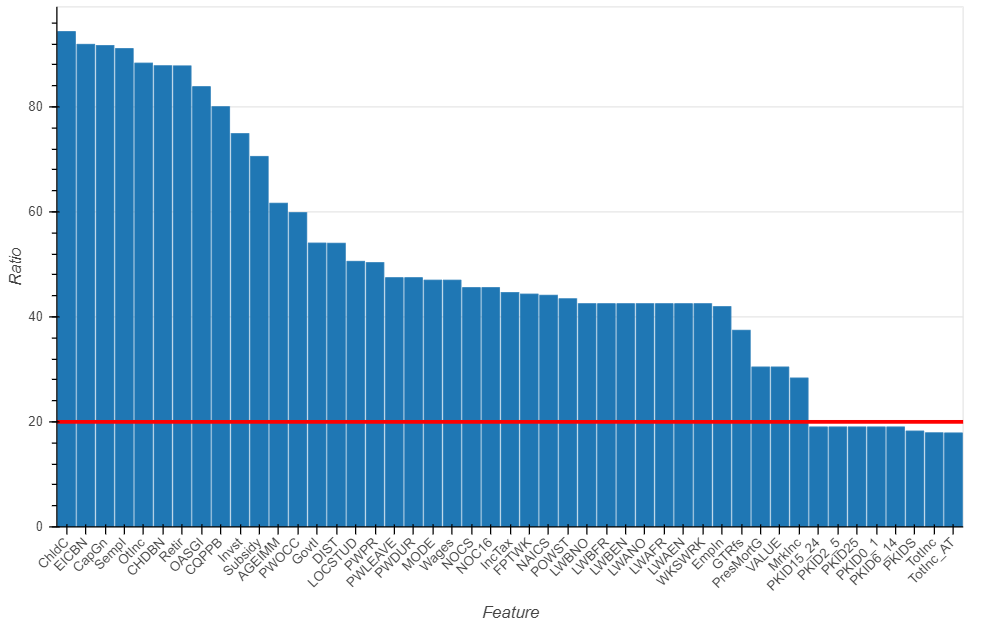
\includegraphics[scale=0.25]{invalid_data_by_feature}
  \centering
  \caption{Invalid data by feature}
  \label{fig:invalid_data}
\end{figure}

The PUMF dataset also contained missing, invalid, or inapplicable values as specified by certain numeric codes (e.g.  88888888) as specified in its accompanying Study Documentation.  The initial preprocessing involved detecting the number of such values in each feature column as a proportion of the total number of entries.  Features which possessed an unusable percentage greater than 20\% were pruned so as to not obscure the analysis by training classifiers on presence of a data feature rather than its content. A subset of the feature's invalid data rates can be seen in figure \ref{fig:invalid_data}.


The initial data analysis also found promising improvements when dropping rows featuring English as a mother tongue.  Removal of these rows lowered the unusable proportion of many features that was thought to provide useful insight, such as AGEIMM (age of immigration) which dropped from 88 to 61 percent unusable.  Although AGEIMM in particular remained unsuitable for the analysis as only a fraction of respondents provided a usable value, a decision was made to remove English mother tongue rows from the dataset with the intention of providing more focused analysis on changes within Canada's non-official language communities, from which shifts to English as a home language were more common than the inverse.

Finally, the data is split into training and testing data sets with 75\% of the data being allocated for training, and the remaining 25\% for testing.

\subsubsection{Imputation}
Since some values in the PUMF data are marked as invalid or unavailable, further preprocessing on the data was required.  As mentioned, data imputation was considered as a remedy for unusable data, but opted against due to the presence of weights attached to each record in the PUMF dataset.  The dataset is meant to balance presenting a representative subset of Canada's demographics while also anonymizing census results which, by Canadian law, are to be withheld from complete public disclosure for 92 years post-response.  As such, each row in the PUMF dataset is a weighted representation of several individuals, listed under the attribute WEIGHT.  Imputation of unusable values, even with the feature's weighted mean as a substitution, was reasoned to be inapplicable without rendering the dataset no longer representative of Canada's demographics.

\subsubsection{Shift Detection}
The process for identifying language shift involves constructing a Boolean feature called \textbf{languageShift}, computed from the MTNNO (mother tongue) and HLANO (home language) attributes.

In the PUMF dataset, both the MTNNO and HLANO features are categorical attributes encoded as a numeric value.  Each feature's encodings are independent and cannot be readily compared, although there exists an intersection between the categories represented within each feature.  Dictionaries for mapping MTNNO and HLANO categories to equivalency classes were manually defined using information outlined in the PUMF Study Documentation file.  These classes include both whole languages such as "Arabic" as well as grouped categories such as "Austro-Asiatic languages".

As the MTNNO categories are less broad and appear to be a superset of the HLANO categories, some categories appear in MTNNO but not HLANO, such as "Uralic" or Korean".  Rather than omitting rows containing these mother tongues, they are categorized under the "All other languages" class.

The value of the languageShift attribute is then defined as the presence of inequivalent class mappings in the MTNNO and HLANO features within a data row.  The reasoning behind this decision is that a difference between mother tongue and home language implies a shift having occurred at some point within an individual's lifetime, with the assumption made being that an individual's mother tongue must at one point have been their home language, possibly only in childhood or even outside of Canada.

If MTNNO can be mapped to HLANO, the languageShift value of a row is false.  If no mapping can be found, the languageShift value will be true.  As with other features in the dataset, the results of the languageShift column are to be interpreted as representative of several individuals.  A row's weight is to be factored into any analysis on or prediction of the languageShift feature.


\subsection{Decision Tree}
The decision tree classifier was build using \textit{scikit-learn}'s implementation, \textit{DecisionTreeClassifier}. The maximum depth of the decision tree was set to be 8 since this is approximately the square root of the number of features being included in the classifier.

The languageShift and WEIGHT attributes are first separated from the dataset to serve as class labels and weights respectively.  MTNNO and HLANO are dropped from the dataset as they are directly involved in the computation of languageShift, for which their effects on a classifier for would be uninteresting.  The remaining attributes in the preprocessed dataset are then to be used as classification features. The features and weights for the training data are then passed into the classifier, with the weights being passed into the \textit{sample weight} parameter of the \textit{fit} function on the decision tree classifier. The class of test samples are predicted using the \textit{predict} function. Finally, the results of the classifier are output in a confusion matrix.

\subsection{Random Forest}

Similarly to the decision tree classifier, the random forest classifier was constructed using \textit{scikit-learn}'s implementation, \textit{RandomForestClassifier}, using 20 estimators and a controlled random state to maintain similar, repeatable results after multiple runs. No maximum depth was specified for the Random Forest classifier.

The classifier is trained on the training data set, along with their weights, then evaluated on the testing data set. The predicted class of test samples is determined using the \textit{predict} function by selecting the class with the highest mean probability estimate across all trees in the random forest. The results are also outputted to a confusion matrix.

\subsection{Naive Bayesian}

The Naive Bayesian classifier was built using \textit{scikit-learn}'s \textit{CategoricalNB} - a Naive Bayes classifier for categorical features. This classifier assumes that each feature has its own categorical distribution. The \textit{fit} method was used to train the classifier on the weighted training data. The \textit{predict} method was used to perform classification on the testing data. The results are also outputted to a confusion matrix.

\section{Analytic Evaluation}

% @TODO fill in
% observations
% - the decision tree and random forest had very similar feature importances, and precision/recal/etc.
%   - this can also be seen in the ROC AUC's
% - the decision tree and random forest were really good at classifying negative class, not so much the positive class
%   - this could be due to the imbalanced nature of the data; there was a lot more negative examples than positive one
% - the NB classifier had decent recall (with a better recall for the positive class), but a poor precision rate for the positive class
%   - in contrast to the decision tree/random forest where the precision was decent in both classes
%   - kinda similar to that one paper (\cite{performance1}), but NB managed to outperform in recall for all classes and precision
% - f1 score for the Naive Bayes all around worse than the decision tree / random forest
% - ROC AUC for NB was noticeably worse
% - the feature importances for DT/RF are pretty intuitive, with the exception of labour force (didn't look at what that is too much though)

\begin{figure}
  \begin{tabular}{lllll}
                  & precision & recall      & f1-score  & support \\
  \textit{False}  & 0.88      & 0.95        & 0.91      & 74204 \\
  \textit{True}   & 0.75      & 0.51        & 0.61      & 20565 \\
  Total           &           & (accuracy)  & 0.86      & 94769 \\\
  \end{tabular}
  \caption{Decision tree metrics}
  \label{fig:decision_tree_metrics}
\end{figure}

\begin{figure}
  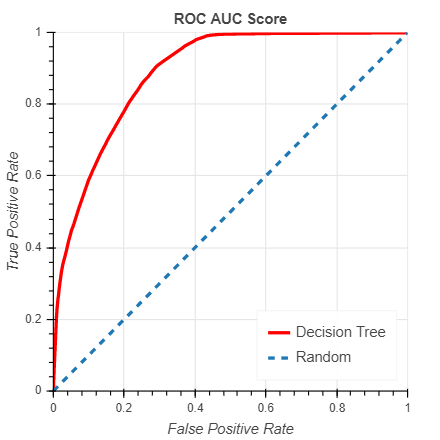
\includegraphics[scale=0.45]{decision_tree_roc}
  \centering
  \caption{Decision tree ROC AUC score}
  \label{fig:decision_tree_roc}
\end{figure}

\begin{figure}
  \begin{tabular}{ll}
    \textbf{Feature}                          & \textbf{Importance} \\
    GENSTAT (Generation status)               & 0.459719 \\
    VisMin (Visible minority status)          & 0.12905 \\
    PR (Province, current)                    & 0.0875603 \\
    POB (Place of birth)                      & 0.0789063 \\
    ETHDER (Ethnic origin)                    & 0.0784669 \\
    IMMCAT5 (Immigration Admission category)  & 0.0324108 \\
    LOC\_ST\_RES (Location of study)          & 0.0279763 \\
    DPGRSUM (Population group)                & 0.0245261 \\
    LFACT (Labour force status)               & 0.0120307 \\
    AGEGRP (Age)                              & 0.0118114 \\   
  \end{tabular}
  \caption{Decision tree feature importances}
  \label{fig:decision_tree_importances}
\end{figure}

\begin{figure}
  \begin{tabular}{lllll}
                  & precision & recall      & f1-score  & support \\
  \textit{False}  & 0.89      & 0.95        & 0.92      & 73875 \\
  \textit{True}   & 0.77      & 0.57        & 0.65      & 20894 \\
  Total           &           & (accuracy)  & 0.87      & 94769 \\\
  \end{tabular}
  \caption{Random forest metrics}
  \label{fig:random_forest_metrics}
\end{figure}

\begin{figure}
  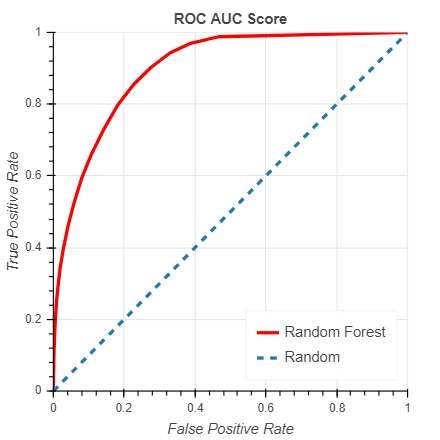
\includegraphics[scale=0.45]{random_forest_roc}
  \centering
  \caption{Random forest ROC AUC score}
  \label{fig:random_forest_roc}
\end{figure}

\begin{figure}
  \begin{tabular}{ll}
    \textbf{Feature}                          & \textbf{Importance} \\
    GENSTAT (Generation status)               & 0.062281 \\
    ETHDER (Ethnic origin)                    & 0.0573086 \\
    PR (Province, current)                    & 0.0523802 \\
    POBM (Mother's POB)                       & 0.048009 \\
    POB (Place of birth)                      & 0.0405777 \\
    POBF (Father's POB)                       & 0.0321791 \\
    VisMin (Visible minority status)          & 0.0253287 \\
    AGEGRP (Age)                              & 0.0240645 \\
    PR5 (Province, 5 years ago)               & 0.0239604 \\
    IMMCAT5 (Immigration admission category)  & 0.0232537
  \end{tabular}
  \caption{Random forest feature importances}
  \label{fig:random_forest_importances}
\end{figure}

\begin{figure}
  \begin{tabular}{lllll}
                  & precision & recall      & f1-score  & support \\
  \textit{False}  & 0.93      & 0.69        & 0.79      & 73954 \\
  \textit{True}   & 0.43      & 0.82        & 0.56      & 20815 \\
  Total           &           & (accuracy)  & 0.72      & 94769 \\\
  \end{tabular}
  \caption{Naive Bayes metrics}
  \label{fig:naive_bayes_metrics}
\end{figure}

\begin{figure}
  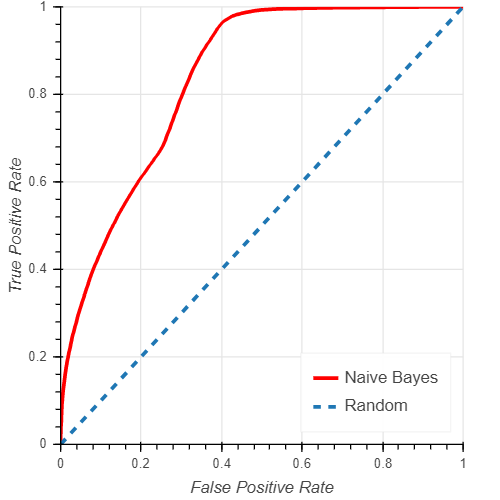
\includegraphics[scale=0.45]{naive_bayes_roc}
  \centering
  \caption{Naive Bayes ROC AUC score}
  \label{fig:naive_bayes_roc}
\end{figure}
% An example of a floating figure using the graphicx package.
% Note that \label must occur AFTER (or within) \caption.
% For figures, \caption should occur after the \includegraphics.
% Note that IEEEtran v1.7 and later has special internal code that
% is designed to preserve the operation of \label within \caption
% even when the captionsoff option is in effect. However, because
% of issues like this, it may be the safest practice to put all your
% \label just after \caption rather than within \caption{}.
%
% Reminder: the "draftcls" or "draftclsnofoot", not "draft", class
% option should be used if it is desired that the figures are to be
% displayed while in draft mode.
%
%\begin{figure}[!t]
%\centering
%\includegraphics[width=2.5in]{myfigure}
% where an .eps filename suffix will be assumed under latex, 
% and a .pdf suffix will be assumed for pdflatex; or what has been declared
% via \DeclareGraphicsExtensions.
%\caption{Simulation Results}
%\label{fig_sim}
%\end{figure}

% Note that IEEE typically puts floats only at the top, even when this
% results in a large percentage of a column being occupied by floats.


% An example of a double column floating figure using two subfigures.
% (The subfig.sty package must be loaded for this to work.)
% The subfigure \label commands are set within each subfloat command, the
% \label for the overall figure must come after \caption.
% \hfil must be used as a separator to get equal spacing.
% The subfigure.sty package works much the same way, except \subfigure is
% used instead of \subfloat.
%
%\begin{figure*}[!t]
%\centerline{\subfloat[Case I]\includegraphics[width=2.5in]{subfigcase1}%
%\label{fig_first_case}}
%\hfil
%\subfloat[Case II]{\includegraphics[width=2.5in]{subfigcase2}%
%\label{fig_second_case}}}
%\caption{Simulation results}
%\label{fig_sim}
%\end{figure*}
%
% Note that often IEEE papers with subfigures do not employ subfigure
% captions (using the optional argument to \subfloat), but instead will
% reference/describe all of them (a), (b), etc., within the main caption.


% An example of a floating table. Note that, for IEEE style tables, the 
% \caption command should come BEFORE the table. Table text will default to
% \footnotesize as IEEE normally uses this smaller font for tables.
% The \label must come after \caption as always.
%
%\begin{table}[!t]
%% increase table row spacing, adjust to taste
%\renewcommand{\arraystretch}{1.3}
% if using array.sty, it might be a good idea to tweak the value of
% \extrarowheight as needed to properly center the text within the cells
%\caption{An Example of a Table}
%\label{table_example}
%\centering
%% Some packages, such as MDW tools, offer better commands for making tables
%% than the plain LaTeX2e tabular which is used here.
%\begin{tabular}{|c||c|}
%\hline
%One & Two\\
%\hline
%Three & Four\\
%\hline
%\end{tabular}
%\end{table}


% Note that IEEE does not put floats in the very first column - or typically
% anywhere on the first page for that matter. Also, in-text middle ("here")
% positioning is not used. Most IEEE journals/conferences use top floats
% exclusively. Note that, LaTeX2e, unlike IEEE journals/conferences, places
% footnotes above bottom floats. This can be corrected via the \fnbelowfloat
% command of the stfloats package.



\section{Conclusion}
% @TODO fill in

% conference papers do not normally have an appendix

\subsection{Future Work}
% @TODO fill in
One aspect that could be improved on in future work is to tweak the hyper parameters for the classifiers via cross validation. For instance, \textit{scikit-learn}'s decision tree classifier implementation allows for setting a maximum depth on the resulting tree. Modifying this value may result in a mire accurate classifier.

Additionally, the 2016 Canadian Census data set contains mostly data indicating a lack of language shift. As a result, the classifiers learn mostly on these negative results, and it may impact the rates for positive results. The weights on the training data could be re-weighted to account for this, but further complications may arise when trying to maintain the data being representative of the Canadian public.

Furthermore, this analysis could be applied over multiple census years. In addition to increasing the amount of data available, adding a temporal dimension could add an interesting aspect to the classifiers, possibly taking historical events into account.

Adding a geographical dimension to the classifiers could identify more granular language shifts in Canadian provinces and territories. It would be interesting to apply the analysis on municipalities such as the City of Winnipeg as well. The Winnipeg open census data portal contains information on language spoken broken down by neighbourhood and ward.

Another interesting metric that could be determined in future work is the conditional probability of each category of each feature influencing the language shift category. For instance, \textit{scikit-learn}'s CategoricalNB classifier implementation contains a feature log prob attribute that returns a 2D array for each feature, which contains the logarithmic probability that each category of the feature influences the language shift category.

% use section* for acknowledgement
\section*{Acknowledgment}


The authors would like to thank the staff at the Elizabeth Dafoe library for giving direction on locating census microdata, and Dr. Carson Leung of the Databases and Data Mining Laboratory at the University of Manitoba for support of this project.


% trigger a \newpage just before the given reference
% number - used to balance the columns on the last page
% adjust value as needed - may need to be readjusted if
% the document is modified later
%\IEEEtriggeratref{8}
% The "triggered" command can be changed if desired:
%\IEEEtriggercmd{\enlargethispage{-5in}}

% references section

% can use a bibliography generated by BibTeX as a .bbl file
% BibTeX documentation can be easily obtained at:
% http://www.ctan.org/tex-archive/biblio/bibtex/contrib/doc/
% The IEEEtran BibTeX style support page is at:
% http://www.michaelshell.org/tex/ieeetran/bibtex/
%\bibliographystyle{IEEEtran}
% argument is your BibTeX string definitions and bibliography database(s)
%\bibliography{IEEEabrv,../bib/paper}
%
% <OR> manually copy in the resultant .bbl file
% set second argument of \begin to the number of references
% (used to reserve space for the reference number labels box)
%\begin{thebibliography}{1}

%\bibitem{IEEEhowto:kopka}
%H.~Kopka and P.~W. Daly, \emph{A Guide to \LaTeX}, 3rd~ed.\hskip 1em plus
%  0.5em minus 0.4em\relax Harlow, England: Addison-Wesley, 1999.

%\end{thebibliography}

\bibliographystyle{IEEEtran}
\bibliography{bare_conf}

% that's all folks
\end{document}


